\documentclass[11pt,a4paper]{article}
\usepackage[margin=24mm]{geometry}
\usepackage[T1]{fontenc}
\usepackage{amsmath,amssymb,amsthm,amscd,mathtools,mathrsfs,array,longtable,booktabs,graphicx,microtype,xurl}
\usepackage[hidelinks,hypertexnames=false]{hyperref}
\allowdisplaybreaks
\emergencystretch=3em
\newtheorem{theorem}{Theorem}[section]
\newtheorem{proposition}[theorem]{Proposition}
\newtheorem{lemma}[theorem]{Lemma}
\newtheorem{corollary}[theorem]{Corollary}
\theoremstyle{definition}\newtheorem{definition}[theorem]{Definition}
\newtheorem{remark}[theorem]{Remark}
\providecommand{\C}{\mathbb C}\providecommand{\R}{\mathbb R}
\providecommand{\Q}{\mathbb Q}\providecommand{\Z}{\mathbb Z}
\providecommand{\N}{\mathbb N}\providecommand{\Spec}{\operatorname{Spec}}
\providecommand{\SpecLat}{\operatorname{Spec}_{\mathrm{lat}}}
\title{Adelic Coefficients on the Full Split-Support Base\\
Prime Transport, Localized Supports, and Synchronization}
\author{Programme derivations with the original human sources cited throughout}
\date{23 September 2026}
\begin{document}\maketitle
This reader constructs the entire divisor-indexed family of the original
Connes--Consani adelic coefficient sheaves and its exact extension to an
arbitrary bounded distributive support lattice. It retains the rational
prime maps, original Haar measures, mixed-prime cohomology, actual
support localizations, and both original-zeta endpoint contributions.
The incoming finite heat/translation construction is applied to those
same sheaves. The different projectors remain visible at support primes
even though their additive group reflections agree. No identification
of the resulting positive quotient metric with Weil's form is assumed.
The complete arguments are CDV1--25, ULC1--18, and CLS1--13.
The appendices retain the support-localization and Mellin proofs used
by them. The source archive also retains the complete predecessor
sources and the unchanged original author archives.
\tableofcontents\clearpage
\begin{figure}[p]\centering
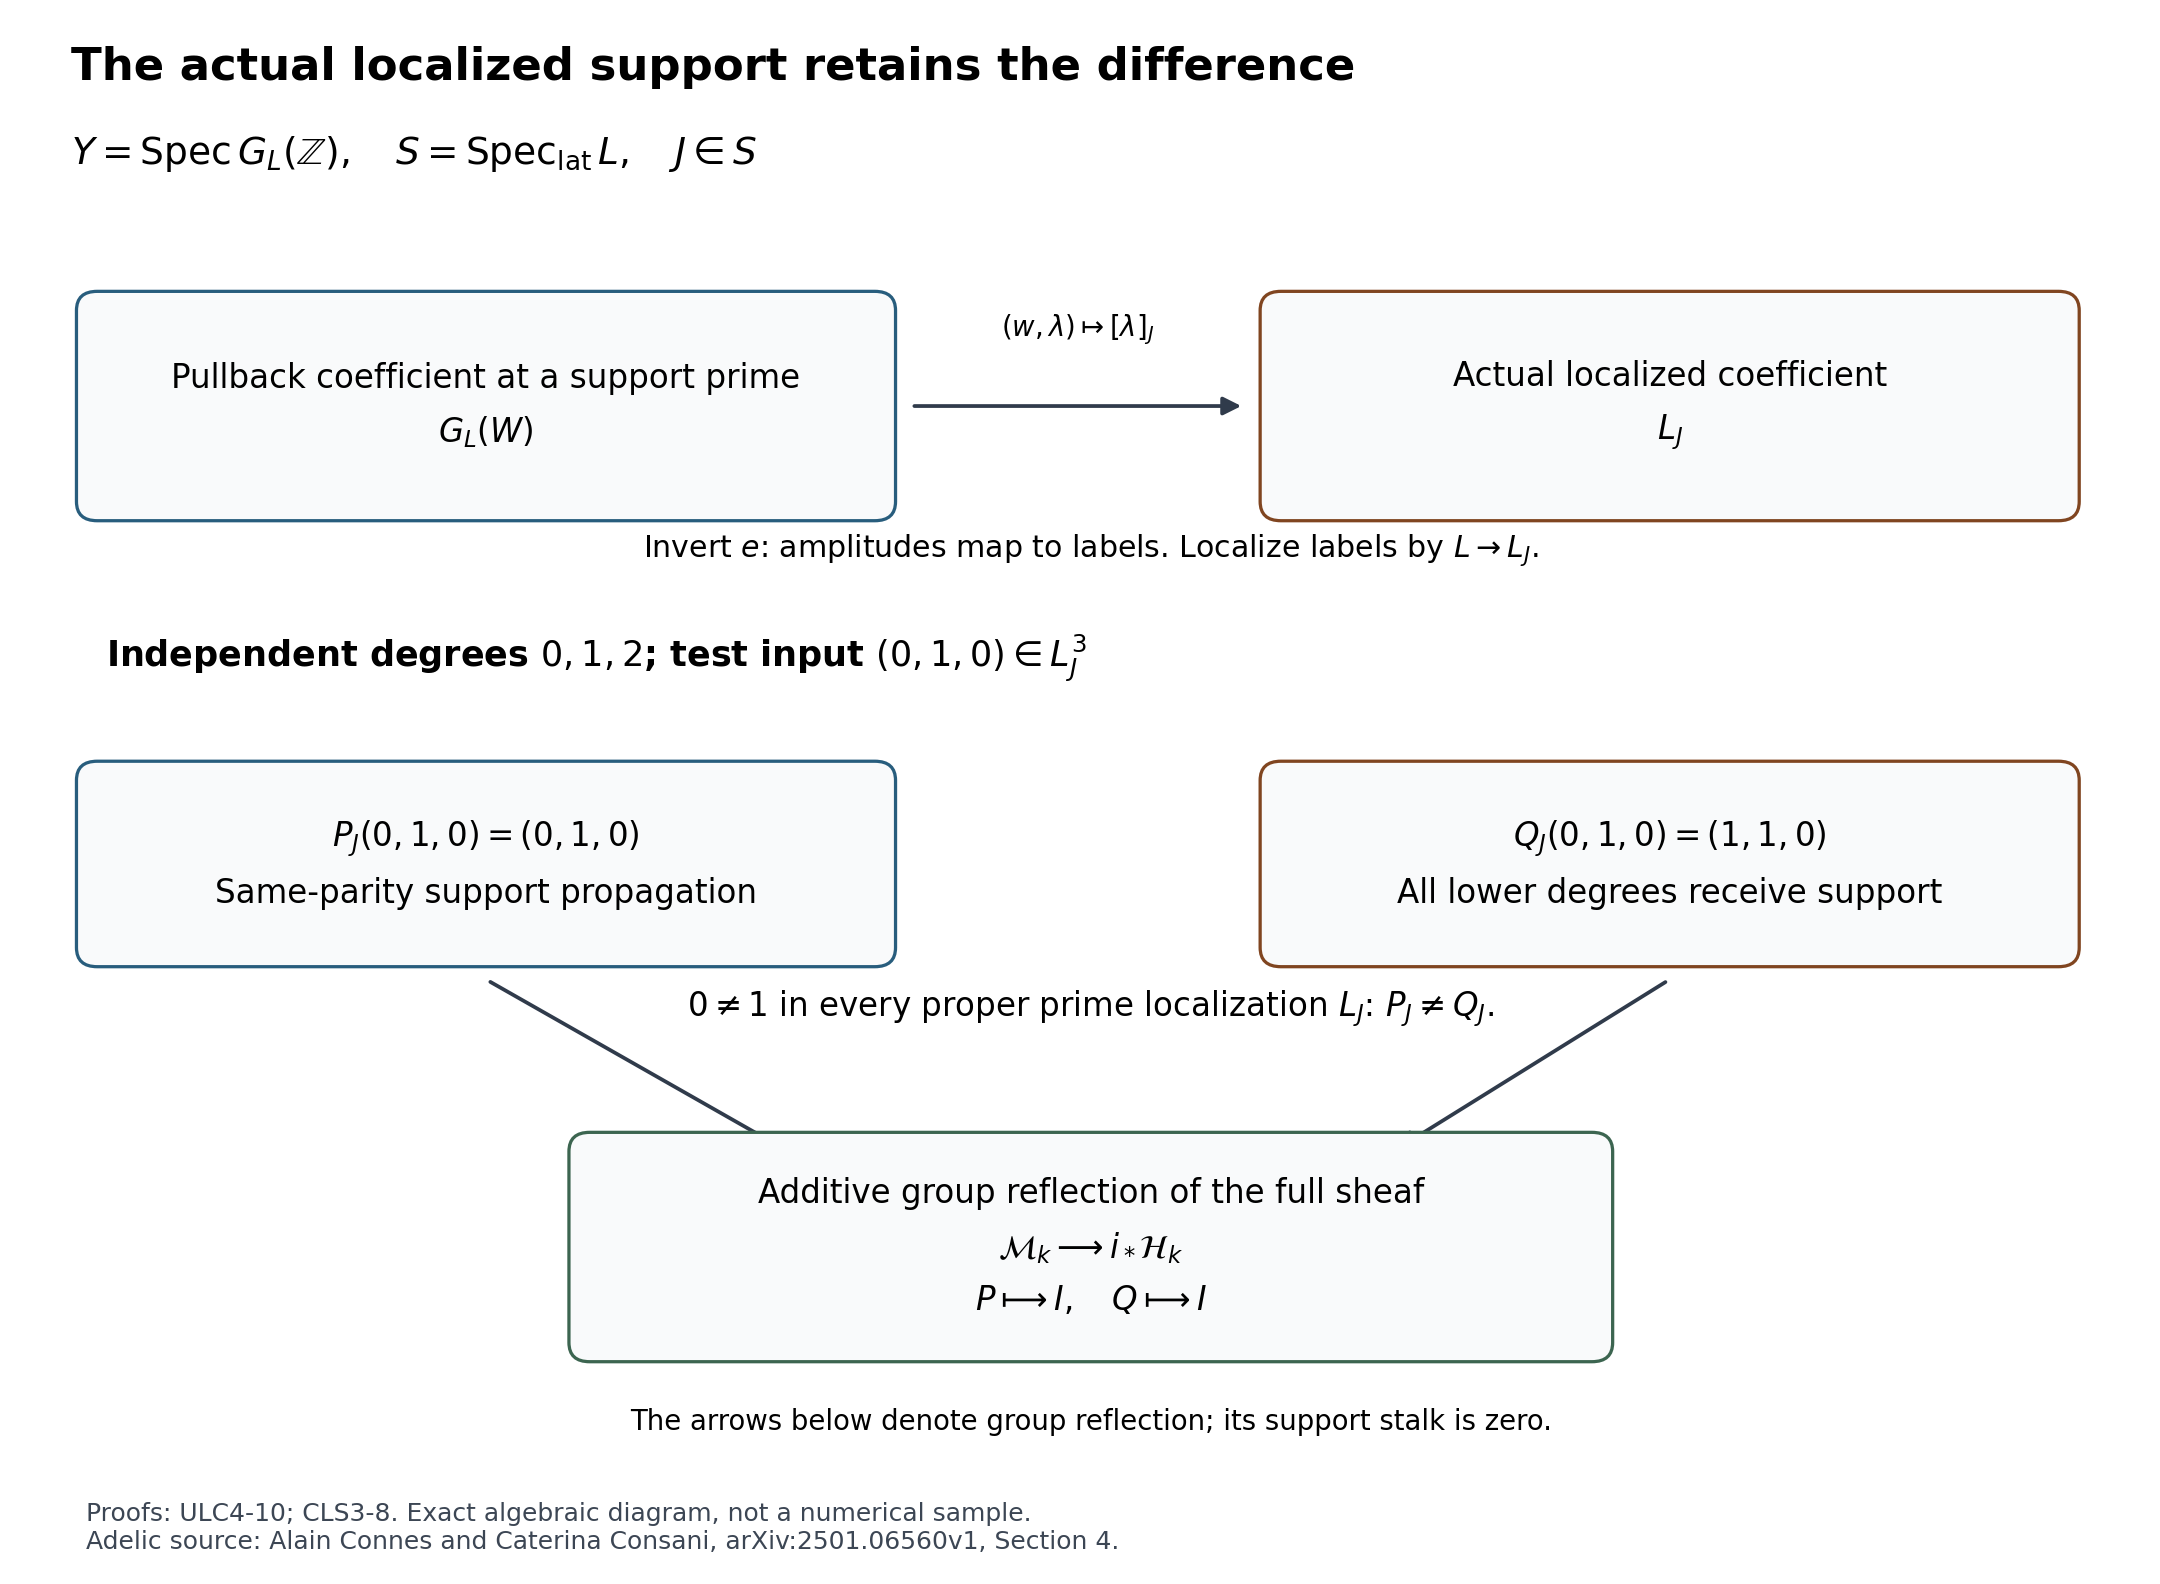
\includegraphics[width=\textwidth]{LOCALIZED_SUPPORT_MAP.png}
\caption{The exact source and support comparisons. The vector
$(0,1,0)$ is a lattice-valued coefficient vector, not a vector of
complex amplitudes. The bottom arrows refer to the amplitude reflection
of the sheaf; at a support point its target is zero. ULC4--10 and
CLS3--8 prove all displayed maps.}
\end{figure}\clearpage

% Complete proof source: CC_DIVISOR_COEFFICIENT_FAMILY.tex
% CDV: exact divisor-indexed extension of CC semilocal coefficients.
\section{All rational-prime translates of the original adelic coefficient sheaf}
\label{sec:cc-divisor-coefficients}

\paragraph{Human source, original object, and scope.}
Alain Connes and Caterina Consani,
\href{https://arxiv.org/abs/2501.06560v1}{\emph{Knots, primes and class
field theory}, arXiv:2501.06560v1}, Section 4, original author file
\texttt{arxiv-pisa.tex}, Lemma \texttt{localv}, Proposition
\texttt{structure}, and Theorem \texttt{structure1}, construct the
semilocal coefficient sheaf using the literal transition vectors
$1_{\mathbb Z_p}$. Their author source, SHA-256
\texttt{249fed347469cfaf6da97915d547c2ca704a4ba21cc339613713e570f14d5cea},
has been read in full in this task. The proof below starts with those
functions and keeps every rational scaling and Haar factor. It extends
the programme calculation CCF8--34, whose complete source is retained,
by making the nonunit-prime defect into a family with invertible maps.
The original scalar function remains $\zeta(s)$; its complete local
integrals are calculated at the end. No identification with a Weil
positive form is assumed.

\subsection{The actual family and its sheaf maps}

Put $X=\operatorname{Spec}\mathbb Z$ and
$V=\mathcal S(\mathbb A_{\mathbb Q})$. Here this Bruhat--Schwartz
space is the algebraic restricted tensor product of the real Schwartz
space and the finite locally constant compactly supported function
spaces, with standard vectors $1_{\mathbb Z_p}$. Thus an element is a
finite sum of tensors with only finitely many nonstandard finite
factors. Let
\begin{equation}\tag{CDV1}
 \mathfrak D=\bigoplus_p\mathbb Z,
 \quad k=(k_p)_p,\quad
 c_{p,k_p}=1_{p^{k_p}\mathbb Z_p},\quad
 N(k)=\prod_p p^{k_p}\in\mathbb Q_{>0}.
\end{equation}
Every product indexed by the support of $k$ is finite. Write
$V^{(p)}$ for the restricted tensor product at every place except $p$,
including the real factor, and set
\begin{equation}\tag{CDV2}
 V_{p,k}=\mathbb Cc_{p,k_p}\otimes V^{(p)}\subset V.
\end{equation}
For $U=X\setminus F$, $F$ a finite set of finite primes, define
\begin{equation}\tag{CDV3}
 \mathcal O_k(U)=\bigcap_{p\notin F}V_{p,k}\subset V,
 \qquad \mathcal O_k(\varnothing)=0.
\end{equation}
All restriction maps for nonempty inclusions are inclusions of these
actual subspaces. Explicitly its sections are the tensors with arbitrary
finite factors at $p\in F$ and the specified $c_{p,k_p}$ at every
other finite prime, with arbitrary real Schwartz factor and finite
linear sums.

Here is a proof of this explicit intersection and of the sheaf property.
For a finite collection of primes define commuting idempotents on $V$
by
\begin{equation}\tag{CDV4}
 P_{p,k}f(x_p,x^{(p)})
 =p^{k_p}c_{p,k_p}(x_p)
                  \int_{p^{k_p}\mathbb Z_p}f(y,x^{(p)})\,dy,
 \qquad \operatorname{vol}(\mathbb Z_p)=1.
\end{equation}
The volume of this ball is $p^{-k_p}$, so $P_{p,k}^2=P_{p,k}$
and its image is exactly $V_{p,k}$. Different $p$ act on different
tensor coordinates and therefore commute. For a given $f$, choose a
finite set containing its nonstandard factors and $\operatorname{supp}k$.
Outside that set the conditions are automatic; inside it, being fixed
by every required projection is equivalent to belonging to the image
of their product. This gives precisely the factors in CDV3.
Every nonempty open in $X$ contains the generic point, so compatible
sections on a covering are the same element $f\in V$. Their local
conditions say exactly that $f\in V_{p,k}$ for every point of the
covered open. This is CDV3, proving existence and uniqueness of gluing.
The generic stalk is $V$, and the stalk at $p$ is $V_{p,k}$ because
every finite set away from $p$ can be removed in its neighbourhoods.
At $k=0$ this is the original Connes--Consani sheaf with its unchanged
transition factors.

The sheaf is an algebra under the original pointwise multiplication:
$c_{p,k_p}^2=c_{p,k_p}$, so products preserve every required local
factor. This statement does not assert a multiplicative structure on
the quotient vector spaces introduced below.

For $r\in\mathbb Q^\times$ write
$d(r)=(v_p(r))_p$ and keep the actual dilation
\begin{equation}\tag{CDV5}
 (\alpha_r f)(x)=f(r^{-1}x),\qquad
 \alpha_r:\mathcal O_k\longrightarrow\mathcal O_{k+d(r)}.
\end{equation}
At $p$, multiplication by the unit part of $r$ fixes every ball, so
$\alpha_r c_{p,k_p}=c_{p,k_p+v_p(r)}$. At all other coordinates the
same formula acts on the actual Schwartz factors. This proves CDV5
on every open and its compatibility with restrictions. Its inverse is
$\alpha_{r^{-1}}$, and $\alpha_r\alpha_q=\alpha_{rq}$. These are
algebra isomorphisms between the specified sheaves. The stabilizer of
the index $k$ consists exactly of $r=\pm1$, by unique factorization
of a rational number. The family indexed by $\mathfrak D$ is retained;
no member is replaced by another without this explicit map.

For crossed-product coefficients retain
\begin{equation}\tag{CDV6}
 B=V\rtimes\mathbb Q^\times,\qquad
 B_{p,k}=\bigoplus_{u:\ v_p(u)=0}V_{p,k}U_u,
 \quad (fU_u)(gU_v)=f\alpha_u(g)U_{uv}.
\end{equation}
The sheaf $\mathcal A_k(X\setminus F)$ is the intersection of the
$B_{p,k}$ for $p\notin F$. The argument proving CDV3 works coefficient
by coefficient because every crossed-product element has a unique
finite sum in the group labels. It yields exactly the coefficient
sheaf $\mathcal O_k$ crossed with the units of $\mathbb Z[F^{-1}]$.
The unit condition makes the pointwise coefficient product preserve
the prescribed local balls. Since rational dilations commute,
\begin{equation}\tag{CDV7}
 \alpha_r^B\left(\sum_u f_uU_u\right)
     =\sum_u\alpha_r(f_u)U_u,
 \qquad\alpha_r^B:\mathcal A_k\xrightarrow{\sim}\mathcal A_{k+d(r)}
\end{equation}
preserves the displayed multiplication, all original group labels,
and every restriction. Its inverse is $\alpha_{r^{-1}}^B$.

\subsection{Every mixed-prime cohomology component}

For either $W=V$ or $W=B$, use $W_{p,k}=V_{p,k}$ or $B_{p,k}$.
Define
\begin{equation}\tag{CDV8}
 D_k(W)=\bigoplus_pW/W_{p,k},\qquad
 \delta_k w=([w]_{p,k})_p,\qquad
 C_k(W)=[W\xrightarrow{\delta_k}D_k(W)].
\end{equation}
The arrow lands in the direct sum: only finitely many primes occur
in $k$, the coefficient tensors, or the nonunit valuations of a group
label. The sheaf sequence
\begin{equation}\tag{CDV9}
 0\longrightarrow\mathcal H_k\longrightarrow c_XW
 \longrightarrow\bigoplus_p i_{p*}(W/W_{p,k})\longrightarrow0
\end{equation}
is exact, where $\mathcal H_k=\mathcal O_k$ or $\mathcal A_k$.
At $p$ it is the quotient sequence and at the generic point its last
term is zero; its kernel on an open is precisely the defining
intersection. The constant sheaf is flasque because all nonempty
opens are connected and its restriction maps are identity maps. The
last sheaf has finite-support sections on every nonempty open:
its generic germ is zero, so a section vanishes on a cofinite
neighbourhood of the generic point, leaving only finitely many closed
points. Its restrictions forget components and are onto. Thus it is
also flasque, and CDV9 computes
\begin{equation}\tag{CDV10}
 H^0(X,\mathcal H_k)=\ker\delta_k,\quad
 H^1(X,\mathcal H_k)=D_k(W)/\delta_kW,\quad
 H^j(X,\mathcal H_k)=0\quad(j\ge2).
\end{equation}
This uses the definition of sheaf cohomology through an acyclic
resolution; flasque sheaves are acyclic for global sections. All
maps and terms of that resolution have been specified.

The complete mixed-place decomposition can be written without altering
the original Haar lengths of the local vectors. Put
\begin{equation}\tag{CDV11}
 E_{p,k}=\left\{f\in\mathcal S(\mathbb Q_p):
                  \int_{p^{k_p}\mathbb Z_p}f=0\right\},\quad
 \mathcal S(\mathbb Q_p)=\mathbb Cc_{p,k_p}\oplus E_{p,k}.
\end{equation}
The two projections are exactly CDV4 and $I-P_{p,k}$. Expanding a
finite tensor gives an algebraic direct sum
\begin{equation}\tag{CDV12}
 V=\bigoplus_{T\ \mathrm{finite}}V_{T,k},\qquad
 V_{T,k}=\mathcal S(\mathbb R)\otimes
       \bigotimes_{p\in T}E_{p,k}\otimes
       \bigotimes_{p\notin T}'\mathbb Cc_{p,k_p}.
\end{equation}
Only finitely many terms occur for any input; projection by the
corresponding finite product of $P_{p,k}$ and $I-P_{p,k}$ proves
uniqueness. A $T$ component survives in $V/V_{p,k}$ precisely when
$p\in T$. For a crossed-product term $V_{T,k}U_u$ it survives
precisely at
$T_u=T\cup\{p:v_p(u)\ne0\}$. Therefore the actual differentials
in CDV8 are the diagonal maps on these components, and
\begin{equation}\tag{CDV13}
\begin{split}
 H^1(X,\mathcal O_k)
  &=\bigoplus_{|T|\ge2}
          V_{T,k}\otimes(\mathbb C^T/\Delta\mathbb C),\\
 H^1(X,\mathcal A_k)
  &=\bigoplus_{u,T:\ |T_u|\ge2}
          V_{T,k}U_u\otimes(\mathbb C^{T_u}/\Delta\mathbb C).
\end{split}
\end{equation}
Indeed an empty marked set has zero target, a one-element set has
surjective diagonal, and for every larger finite set the cokernel is
exactly its marked coordinates modulo the diagonal. This proves
CDV13 by actual component maps, rather than dimension counting.

Every rational dilation induces a chain isomorphism
\begin{equation}\tag{CDV14}
 C_k(W)\xrightarrow{\alpha_r}C_{k+d(r)}(W),\qquad
 [w]_{p,k}\longmapsto[\alpha_rw]_{p,k+d(r)},
\end{equation}
with group labels unchanged in the crossed product. Well-definedness
follows from CDV5 and CDV7, and commutation with $\delta$ follows
componentwise. The inverse is the corresponding map for $r^{-1}$.
The local projections conjugate exactly:
$\alpha_rP_{p,k}\alpha_{r^{-1}}=P_{p,k+d(r)}$.
This follows either from their ranges and orthogonality, or directly
from the change of variables in CDV4. Hence every mixed component
$T$, every marked prime, and every diagonal relation is transported
by CDV14. No cohomology component is dropped in this prime action.

\subsection{The original positive metric and the nonunit defect}

The additive adelic Haar measure is the original product of $dx$ at
infinity and measures with $\operatorname{vol}(\mathbb Z_p)=1$.
In particular
\begin{equation}\tag{CDV15}
 \|c_{p,k_p}\|^2=p^{-k_p},\qquad
 \|\alpha_rf\|^2=|r|_\infty\prod_p p^{-v_p(r)}\|f\|^2=\|f\|^2.
\end{equation}
The product formula here follows immediately by writing
$r=\pm\prod p^{v_p(r)}$. Every factor in the preceding product
is retained. The quotient $V/V_{p,k}$ is isometrically represented
by $(I-P_{p,k})V$, since CDV4 is the original Haar orthogonal
projection. Equip $D_k(V)$ with the sum of these squared quotient
norms. In $D_k(B)$, at a coefficient with $v_p(u)=0$ use this
projection, and at $v_p(u)\ne0$ use its full original Haar norm;
sum over the finite coefficient and prime labels. CDV14 is an
isometry for these metrics, by CDV15 and the conjugation identity.

Completion and quotient do not delete the mixed arithmetic part.
The orthogonal expansion CDV12, retaining all factors $p^{-k_p}$,
gives
\begin{equation}\tag{CDV16}
 \overline{D_k(V)}/\overline{\delta_kV}
 =\widehat{\bigoplus}_{|T|\ge2}\overline{V_{T,k}}
                  \otimes(\Delta\mathbb C)^\perp.
\end{equation}
To verify the closures, finite tensors are dense in each Hilbert
summand by its definition. Each finite collection of diagonal
components is the image of their sum in $V$. Conversely the
bounded orthogonal projection on every marked-coordinate factor
annihilates $\delta_kV$, so its closure has no component outside
the diagonal. These two inclusions prove the displayed equality.
On $\mathbb C^T$ the diagonal projection is exactly
$(c_p)_p\mapsto(|T|^{-1}\sum_pc_p)_p$; its denominator remains.
The same proof with $T_u$ gives CDV16 for $B$ with every $U_u$
retained. The original algebraic quotient injects into the Hilbert
quotient, since a finite vector has zero orthogonal projection
exactly when its components were already diagonal. These are
particular positive quotient metrics, not an identification with
the original Weil trace.

If instead one insists on the fixed target $V/V_{p,k}$, the
nonunit action has a nonzero defect. For an integer $m$ and
$f=c_{p,k_p}\otimes g$, its representative is
\begin{equation}\tag{CDV17}
 (I-P_{p,k})\alpha_{p^m}f
 =\left(c_{p,k_p+m}-p^{-\max(0,m)}c_{p,k_p}\right)
                        \otimes\alpha_{p^m}^{(p)}g.
\end{equation}
Indeed the overlap of the two balls has volume
$p^{-\max(k_p,k_p+m)}$ and CDV4 supplies the multiplier
$p^{k_p}$. Taking its original squared norm gives
\begin{equation}\tag{CDV18}
 \|(I-P_{p,k})\alpha_{p^m}f\|^2
 =p^{-k_p}\bigl(1-p^{-|m|}\bigr)\|g\|^2.
\end{equation}
For $m\ge0$ the finite local squared norm is
$p^{-k_p}(p^{-m}-p^{-2m})$; for $m<0$ it is
$p^{-k_p}(p^{-m}-1)$. The other places contribute $p^m$
by the same product formula, yielding CDV18 in both cases.
It vanishes exactly at $m=0$ for nonzero $g$. Thus the
obstruction to a fixed-space endomorphism is a calculated vector;
CDV14 constructs the invertible action on its actual target family.

\subsection{Fourier maps with every local scalar retained}

Use the conductor-$\mathbb Z_p$ additive character at $p$ and
$e^{-2\pi ixy}$ at infinity. Character orthogonality proves
\begin{equation}\tag{CDV19}
 \widehat{c_{p,k_p}}=p^{-k_p}c_{p,-k_p}.
\end{equation}
The annihilator of $p^{k_p}\mathbb Z_p$ is
$p^{-k_p}\mathbb Z_p$: on it the integral is the ball volume;
off it, translating by a point on which the character is nontrivial
forces the integral to be zero. Tensoring gives a vector-sheaf
isomorphism $\mathcal F:\mathcal O_k\to\mathcal O_{-k}$.
Its inverse is Fourier followed by $x\mapsto-x$; this follows
from Fourier inversion on the real Schwartz factor and character
orthogonality on finite local quotients. In semilocal coordinates
the transition includes the full scalar
$\prod_{p\notin F}p^{-k_p}$; it is not the bare map replacing
each standard vector by $c_{p,-k_p}$.

On the original crossed-product multiplication the target is
convolution, and the exact isomorphism is
\begin{equation}\tag{CDV20}
 \sum_u f_uU_u\longmapsto\sum_u\widehat f_uU_{u^{-1}},\qquad
 \mathcal F\alpha_r=\alpha_{r^{-1}}\mathcal F,
 \quad\mathcal F\vartheta_\lambda
                  =\lambda\vartheta_{\lambda^{-1}}\mathcal F.
\end{equation}
Here $\vartheta_\lambda$ acts only on the real coordinate by
$x_\infty\mapsto\lambda^{-1}x_\infty$, $\lambda>0$.
The last two equalities follow by change of variables in the Fourier
integrals; the rational product of moduli is $1$, the real modulus
is $\lambda$. Fourier of a pointwise product is convolution by
Fubini on these functions. Therefore the image of
$f\alpha_u(g)U_{uv}$ is
$\widehat f*\alpha_{u^{-1}}(\widehat g)U_{u^{-1}v^{-1}}$,
which is exactly the target product. It preserves the nonunit
valuation conditions and takes $k$ to $-k$.
For example the image vector $p^{-k_p}c_{p,-k_p}$ is a
convolution idempotent: its convolution square is
$p^{-2k_p}p^{k_p}c_{p,-k_p}$, equal to itself. This verifies
why the retained scalar matters to the algebra map.
All these arrows induce the specified chain and cohomology maps
because they send each local coefficient subspace to its target.

\subsection{Original zeta and the two endpoint functionals}

For $a>0$ define the actual tensor
\begin{equation}\tag{CDV21}
 f_{k,a}(x)=e^{-\pi(x_\infty/a)^2}\prod_p c_{p,k_p}(x_p).
\end{equation}
The two additive moments, computed in the original measures, are
\begin{equation}\tag{CDV22}
 f_{k,a}(0)=1,\qquad \int_{\mathbb A}f_{k,a}(x)\,dx
                         =a\prod_pp^{-k_p}=a/N(k).
\end{equation}
The real Gaussian integral is $a$ by substitution; the finite
integrals are exactly the ball volumes. Thus these are separate
endpoint data, not both replaced by one. Rational dilation gives
$\alpha_rf_{k,a}=f_{k+d(r),|r|a}$, and real scaling gives
$\vartheta_\lambda f_{k,a}=f_{k,\lambda a}$. CDV22 then proves
that the rational map preserves both moments whereas the real map
multiplies only the integral moment by $\lambda$.

For each finite prime use multiplicative Haar measure with
$\operatorname{vol}^{\times}(\mathbb Z_p^\times)=1$, and at
infinity use $dx/|x|$. For $\operatorname{Re}s>1$, define the
adelic multiplicative integral as the absolutely convergent product
of its local integrals. Their complete evaluation is
\begin{equation}\tag{CDV23}
\begin{split}
 \int_{\mathbb Q_p^\times}c_{p,k_p}(x)|x|_p^s\,d^\times x
   &=\sum_{j=k_p}^\infty p^{-js}
     =\frac{p^{-k_ps}}{1-p^{-s}},\\
 \int_{\mathbb R^\times}e^{-\pi(x/a)^2}|x|^s\frac{dx}{|x|}
   &=a^s\pi^{-s/2}\Gamma(s/2),\\
 Z(f_{k,a},s)
   &=a^sN(k)^{-s}\pi^{-s/2}\Gamma(s/2)\zeta(s).
\end{split}
\end{equation}
For the first line partition the support into annuli
$p^j\mathbb Z_p^\times$; multiplicative invariance makes each
annulus have measure $1$. The geometric series converges for
$\operatorname{Re}s>0$. For the second integrate over both signs
and substitute $y=\pi(x/a)^2$; the factor of two and the
Jacobian give exactly the displayed Gamma factor. At the global
step $\sum_pp^{-\operatorname{Re}s}<\infty$ bounds the product.
Unique prime factorization identifies its absolutely convergent
expansion with $\sum_{n\ge1}n^{-s}=\zeta(s)$. Hence the original
function is recovered, with every factor shown, by
\begin{equation}\tag{CDV24}
 \zeta(s)=a^{-s}N(k)^s\frac{\pi^{s/2}}{\Gamma(s/2)}
                         Z(f_{k,a},s).
\end{equation}
No endpoint polynomial $s(s-1)$ was inserted into the arithmetic
function. Meromorphic continuation here uses the original-zeta
formula ZTC10 with its separate $1/(s-1)$ and $-1/s$ terms.
For the actual rational map in CDV22, both $a$ and $N(k)$ are
multiplied by $|r|$, so their two factors in CDV23 cancel exactly.
Changing only the finite-place ball would leave $p^{-ms}$ and
would be a different arithmetic operation. This is the full prime
and archimedean comparison behind that cancellation.

\subsection{Full lattice coefficients and their actual limits}

Let $L$ be any nontrivial bounded distributive lattice, and retain
$G_L(W)=\{(0,\lambda):\lambda\in L\}\cup(W\times\{1_L\})$.
Every linear map above has the exact lift
$(w,\lambda)\mapsto(Tw,\lambda)$. Addition uses label join and
scalar multiplication label meet; substitution proves compatibility
and shows that zeros of amplitudes do not delete their labels.
Every inverse already displayed lifts by the same formula.
In particular the quotient congruence is exactly
the following $G_L(\mathbb C)$-semimodule congruence; it is not
a quotient-algebra assertion, since $W_{p,k}$ need not be an ideal:
\begin{equation}\tag{CDV25}
 (w,\lambda)\sim(w',\lambda')
 \ \Longleftrightarrow\ \lambda=\lambda'\ \hbox{and}\ w-w'\in W_{p,k},
 \qquad G_L(W)/{\sim}\cong G_L(W/W_{p,k}).
\end{equation}
Its classes are the fibres of the surjective quotient map;
the relation is compatible with both operations since $W_{p,k}$
is a vector subspace. Direct-sum formulas lift with one common
label, not independently chosen labels on the target factors.
For sheaves the sectionwise construction is sheafified; stalks are
$G_L(\mathcal H_{k,x})$. To verify that description, filtered
colimits commute with the carrier construction: a nonzero amplitude
is represented with top label; a labelled zero is represented by
that same labelled zero at any stage, and equality is exactly
equality at a later stage together with equality of labels.
Sheafification leaves stalks unchanged. All maps and inverse
identities therefore survive sheafification.

This coefficient lift does not remove the supported-zero prime.
For $G_L(\mathbb Z)$ its element $e=(0,1_L)$ generates the ideal
of all labelled zeros, since $e(a,\lambda)=(0,\lambda)$.
The amplitude map $q:G_L(\mathbb Z)\to\mathbb Z$ sends this
ideal to $(0)$, and $q^{-1}(0)=(e)$ is prime: if $q(x)q(y)=0$
in the domain $\mathbb Z$, one amplitude is zero. This proves
the actual prime statement, retaining every zero label. The
arithmetic prime $(p)$ similarly has inverse image $q^{-1}(p)$
containing $(e)$ strictly. The rest of the support spectrum and
its stalks remain part of the base; no scalar Mellin evaluation
is asserted to recover them. CDV25 specifies the coefficient
maps that can be applied on that base, while its full support
cohomology requires the sheaf extension constructed separately.

\clearpage

% Complete proof source: ARBITRARY_SUPPORT_CC_COEFFICIENTS.tex
% ULC: arbitrary support spectrum, actual localized coefficients, and CC family.
\section{The Connes--Consani coefficient family on the actual arbitrary support base}
\label{sec:arbitrary-support-cc}

\paragraph{Sources and scope.}
The human adelic source is Alain Connes and Caterina Consani,
\href{https://arxiv.org/abs/2501.06560v1}{\emph{Knots, primes and class
field theory}}, Section 4, author-source labels \texttt{localv},
\texttt{structure}, and \texttt{structure1}. CDV1--25 supplies the
complete divisor-indexed extension and proofs, retaining the original
local Haar measures and real factor. FSC1--9 and FSC33--34 supply the
support topology and localization maps; their full proofs accompany
this chapter. Their foundation is the
\href{https://github.com/KokunoYumeto/zeta-function-research-reader/blob/a2851f9eb352e7e4376bc629de86fa4ed9c1c434/workbenches/splitzero-tandem/foundations/split-support-geometry-v11/split_support_geometry_arithmetic_curve_v11.tex}{pinned Split Support Geometry v11 source},
Definition \texttt{def:lattice-split} and the subsequent ideal and prime
classification. This chapter derives the actual coefficient modules
and the arbitrary-support cohomology comparison. It does not identify
an idempotent semimodule with an abelian sheaf.

\subsection{The base and its two types of open}
Let $L$ be a nontrivial bounded distributive lattice, possibly infinite,
and retain
\begin{equation}\tag{ULC1}
 X=\operatorname{Spec}\mathbb Z,\quad
 S=\operatorname{Spec}_{\mathrm{lat}}L,\quad
 Y=\operatorname{Spec}G_L(\mathbb Z)=S\sqcup X.
\end{equation}
The points of $S$ are proper prime lattice ideals $J$, represented in
the semiring spectrum by $\{(0,\lambda):\lambda\in J\}$. The points
of $X$ are $q^{-1}(\mathfrak p)$, where $q(a,\lambda)=a$.
An ideal containing a top-supported element contains $e=(0,1_L)$:
add that element to its product with $(-1,1_L)$. Multiplication by
$e$ then supplies all labelled zeros. Its amplitudes form a ring
ideal. Every ideal without a top-supported element is a proper lattice
ideal of zero labels. Primality is respectively ring or meet primality.
This proves the stated partition of the points. Its basic opens are
$D((n,1_L))=S\cup D_X(n)$ for $n\ne0$ and
$D((0,\lambda))=D_L(\lambda)\subset S$.
Consequently every open of $Y$ is either an open $V\subset S$ or
\begin{equation}\tag{ULC2}
 W_U=S\cup U\quad(\varnothing\ne U\subset X\text{ open}).
\end{equation}
All nonempty opens of $X$ contain the generic point $\eta$ and are
cofinite. Write $i:X\hookrightarrow Y$ and $j:S\hookrightarrow Y$.
The map $r:Y\to X$ is the identity on $X$ and sends every point of
$S$ to $\eta$. It is continuous since $r^{-1}U=W_U$ for nonempty
$U$, and $ri=\mathrm{id}$. Nontriviality of $L$ implies $S\ne\varnothing$
by prime-ideal separation, whose proof is included in FSC6.

The actual structure sheaf has
\begin{equation}\tag{ULC3}
 \mathcal O_Y(W_U)=G_L(\mathcal O_X(U)),\quad
 \mathcal O_Y|_S=\mathcal O_S,\quad
 \mathcal O_S(D_L(\lambda))=\downarrow\lambda,\quad
 (\mathcal O_S)_J=L_J.
\end{equation}
Here $L_J$ is the localization with equality
$[\lambda]_J=[\mu]_J$ precisely when
$\lambda\wedge\nu=\mu\wedge\nu$ for some $\nu\notin J$.
On basic support opens the restriction is $a\mapsto a\wedge\lambda$.
Finite covers glue by joins and distributivity; compactness of the
basic opens reduces an arbitrary covering to this assertion.
On $W_U$, the generic arithmetic germ fixes one rational amplitude
and one label, and the amplitude must be regular at every included
prime; this proves the first formula. Restriction to $S$ retains
the label and localizes it. These observations prove ULC3 with the
original structure sheaf, not a constant substitute.

\subsection{The actual localized coefficient semimodule}
Let $\mathcal H_k$ be either CDV's $\mathcal O_k$ or $\mathcal A_k$
on $X$, with generic complex vector space $W=V$ or $B$ and stalks
$W_{p,k}$. It is an $\mathcal O_X$-module by multiplication by the
rational scalar in each regular section. This scalar action preserves
each complex subspace and every restriction.

Define a sheaf $\mathcal M_k$ of $\mathcal O_Y$-semimodules by
\begin{equation}\tag{ULC4}
 \mathcal M_k(W_U)=G_L(\mathcal H_k(U)),\qquad
 \mathcal M_k(V)=\mathcal O_S(V)\quad(V\subset S).
\end{equation}
On arithmetic opens, restrictions restrict the amplitude and keep
the label. Restriction from $W_U$ to a support open sends
$(w,\lambda)$ to the section represented by $\lambda$, with all its
localizations retained. On support opens use the actual restrictions
of $\mathcal O_S$. The scalar operation on an arithmetic open is
$(a,\mu)(w,\lambda)=(aw,\mu\wedge\lambda)$ and addition uses join.
On support opens scalar operation is meet and addition is join.
All these formulas commute with restrictions.

Here is a direct gluing proof. A cover of $W_U$ has some arithmetic
members $W_{U_a}$ covering $U$. Any two have nonempty arithmetic
intersection, so compatible sections have one common label and their
amplitudes glue in $\mathcal H_k$. A nonzero glued amplitude has
nonzero restriction somewhere, hence top label. The arithmetic member
already covers all of $S$; compatibility forces each purely support
member to carry precisely the restriction of that common label.
Thus the glued section is unique and belongs to ULC4. Covers of a
support open glue in $\mathcal O_S$. This proves the sheaf assertion
and the scalar operations on the original carrier. Its stalks are
\begin{equation}\tag{ULC5}
 (\mathcal M_k)_\eta=G_L(W),\qquad
 (\mathcal M_k)_p=G_L(W_{p,k}),\qquad
 (\mathcal M_k)_J=L_J.
\end{equation}
The first two follow by the filtered neighbourhood colimits and CDV's
stalk descriptions. At $J$ the neighbourhoods contained in $S$ are
cofinal and give the last formula.

This is the actual localization of the coefficient carrier at support.
For every $w\in W$, multiplication by $e$ sends $(w,\lambda)$ to
$(0,\lambda)$. Inverting the idempotent $e$ makes it the unit, so
\begin{equation}\tag{ULC6}
 G_L(W)[e^{-1}]\simeq L,
 \qquad G_L(W)_{P_J}\simeq L_J.
\end{equation}
To verify the first isomorphism rather than only its surjectivity,
the support map has the section $\lambda\mapsto(0,\lambda)$;
every localized element equals its product with $e$, and equality
of these zero labels is unchanged by multiplication by $e$.
Further inversion of the zero labels outside $J$ gives exactly
the relation in ULC3. Every top-supported nonzero integer already
maps to the unit of that localized lattice. No additional relation
arises from those integers. This proves the second isomorphism.

Retain separately the inverse-image coefficient sheaf
\begin{equation}\tag{ULC7}
 \mathcal P_k=r^{-1}G_L(\mathcal H_k),\qquad
 \mathcal P_k\longrightarrow\mathcal M_k.
\end{equation}
Here $G_L(\mathcal H_k)$ on $X$ has the section formula used in
ULC4; its sheaf proof follows from the same common-generic-point
argument. The arrow is the identity on arithmetic opens. On a support
open it sends a locally constant section of $G_L(W)$ to its support
label and then to its localizations in $\mathcal O_S$.
It commutes with restrictions because a section on $W_U$ restricts
in $\mathcal P_k$ to its constant generic germ, whereas in
$\mathcal M_k$ it restricts to its localized label. Its stalk map is
the identity at arithmetic points and
\begin{equation}\tag{ULC8}
 G_L(W)\longrightarrow L\longrightarrow L_J,
 \qquad (w,\lambda)\longmapsto\lambda\longmapsto[\lambda]_J
\end{equation}
at a support prime. It is surjective on stalks. The precise fibre
relation at $J$ is existence of $\nu\notin J$ with
$\lambda\wedge\nu=\mu\wedge\nu$; amplitudes impose no further
condition. This comparison is linear over the corresponding sheaf
map $r^{-1}G_L(\mathcal O_X)\to\mathcal O_Y$.
One cannot make the unchanged $\mathcal P_k$ into an
$\mathcal O_Y$-semimodule extending that coefficient action at a
support point: $e$ is a unit there but kills each nonzero amplitude
under the original action. The map ULC8 computes the required
localization rather than assuming it away.

\subsection{Retaining the support ideal and the exact amplitude reflection}
Let $\mathcal D=j_*\mathcal O_S$. Its sections on $W_U$ are $L$
and its sections on $V\subset S$ are $\mathcal O_S(V)$.
There are actual semimodule maps
\begin{equation}\tag{ULC9}
 \mathcal D\xrightarrow{z}\mathcal M_k
 \xrightarrow{\sigma}\mathcal D,\quad\sigma z=\mathrm{id},
 \qquad q:\mathcal M_k\longrightarrow i_*\mathcal H_k.
\end{equation}
On $W_U$, $z(\lambda)=(0,\lambda)$, $\sigma(w,\lambda)=\lambda$,
and $q(w,\lambda)=w$. On support opens the first two maps are the
identity, and the last map has zero target. On $\mathcal D$ the
scalar action is induced by $\mathcal O_Y\to\mathcal D$; on the
amplitude target it is induced by $\mathcal O_Y\to i_*\mathcal O_X$.
These formulas prove compatibility with both operations and every
restriction. They give
\begin{equation}\tag{ULC10}
 e\mathcal M_k=z\mathcal D=q^{-1}(0),\qquad
 \mathcal M_k/\!\sim_{z\mathcal D}\ \simeq i_*\mathcal H_k,
\end{equation}
where $x\sim_{z\mathcal D}y$ means locally
$x+z(u)=y+z(v)$ for support sections $u,v$.
Indeed multiplication by $e$ is precisely $z\sigma$. Two sections
$(w,\lambda),(w',\mu)$ on $W_U$ with equal amplitude obey
$(w,\lambda)+z(\mu)=(w',\mu)+z(\lambda)$. Conversely adding
zero-amplitude sections cannot change the amplitude. On a support
open the entire module is $z\mathcal D$. The map $q$ is onto
on sections, using $(w,1_L)$ as a lift. This proves the quotient
description, including its original congruence.

The sheaf associated with additive group completion of $\mathcal M_k$
is exactly $i_*\mathcal H_k$. Every additive map to a sheaf of
abelian groups kills each idempotent zero label because $z+z=z$.
It then identifies the two sections in the preceding displayed
relation and factors uniquely through $q$. Conversely the target
is already an abelian sheaf, and each $w$ is in the image. This
proves the universal property locally and hence for sheaves.
It does not identify $\mathcal M_k$ itself with its group completion.
The retract $z\mathcal D$, all its localized labels, and the map
ULC8 remain explicit parts of the original object.

The image of $(q,\sigma)$ inside
$i_*\mathcal H_k\times\mathcal D$ has on $W_U$ the exact constraint
$w\ne0\Rightarrow\lambda=1_L$ and has the whole support factor
on support opens. It is injective on every stalk by ULC5. Thus an
unrestricted direct product is not the original carrier.

\subsection{Cohomology for an arbitrary support spectrum}
For any abelian sheaf $F$ on $Y$ there is a natural isomorphism
\begin{equation}\tag{ULC11}
 r_*F\simeq i^{-1}F.
\end{equation}
The map is induced by restriction from $W_U$ to neighbourhoods
of $U$ along $i$. Its stalk at $x\in X$ is the identity on
$F_x$: all neighbourhoods of $x$ in $Y$ are exactly the $W_U$
for neighbourhoods $U$ in $X$. This proves the isomorphism and
shows that $r_*$ is exact. It preserves injectives because its
left adjoint $r^{-1}$ is exact. Since
$\Gamma(Y,F)=\Gamma(X,r_*F)$, an injective resolution gives
\begin{equation}\tag{ULC12}
 R\Gamma(Y,F)\simeq R\Gamma(X,i^{-1}F).
\end{equation}
For $F=r^{-1}\mathcal H_k$, the right side is represented by the
actual CDV complex
\begin{equation}\tag{ULC13}
 C_k=[W\xrightarrow{\delta_k}D_k],\quad
 D_k=\bigoplus_p W/W_{p,k},\quad
 \delta_kw=([w]_{p,k})_p.
\end{equation}
For $F=i_*\mathcal H_k$, the same conclusion follows either
from ULC11--12 or from the exactness of closed-embedding direct
image. Consequently the amplitude reflection in ULC10 has
$H^1=D_k/\delta_kW$, including every mixed-prime summand of
CDV13, and vanishes in degrees at least two. No finiteness of
$L$ has been used.

There is more information in the relative comparison for the
\emph{inverse-image vector sheaf} $r^{-1}\mathcal H_k$.
Its restriction to $S$ is the constant sheaf $c_SW$, because
$r|_S$ factors through $\eta$. This is not the support restriction
$\mathcal O_S$ of the original semimodule $\mathcal M_k$.
For clarity define an explicit acyclic resolution of $c_SW$ as
follows. For an abelian sheaf $E$ put
$T(E)(V)=\prod_{x\in V}E_x$ with projection restrictions.
This is a sheaf and is flasque; the germ map $E\to T(E)$ is
injective. Set $E_0=c_SW$, $E_{n+1}=\operatorname{coker}(E_n\to T(E_n))$,
and use the composites $T(E_n)\to E_{n+1}\to T(E_{n+1})$.
The resulting sheaf sequence is exact by its kernel and cokernel
definitions, and all its terms are flasque. Let $B^n=\Gamma(S,T(E_n))$
with differential $d_B$. Then $B^\bullet$ computes
$R\Gamma(S,c_SW)$. This construction retains every infinite
product over the actual points of $S$.

The constant section gives $c:W\to\ker(d_B:B^0\to B^1)$.
The relative cohomology with support in the closed arithmetic
stratum is computed by
\begin{equation}\tag{ULC14}
 W\xrightarrow{d^0}D_k\oplus B^0\xrightarrow{d^1}B^1
 \xrightarrow{-d_B}B^2\xrightarrow{-d_B}\cdots,
 \quad d^0w=(\delta_kw,cw),\quad d^1(d,b)=-d_Bb.
\end{equation}
Here degrees start at zero. To justify the relative comparison,
take an injective resolution on $Y$. Its restrictions to the open
$S$ are injective since extension by zero is an exact left adjoint.
Each injective sheaf is flasque, so restriction of its global
sections to $S$ is onto. The kernel complex therefore computes
sections with support in $X$, and the short exact sequence of
complexes yields the fibre of global restriction. Apply the
CDV flasque resolution to $r^{-1}\mathcal H_k$: inverse image
is exact, its constant first term is $c_YW$, and its closed-prime
term has zero restriction to $S$. These terms are acyclic for
global sections by ULC12, whose direct images are precisely the
two CDV flasque terms. Restriction of this resolution to $S$
has just $c_SW$ in degree zero. Its comparison with the displayed
resolution $B^\bullet$ is the constant germ map in degree zero
and zero in degree one. Thus the fibre complex, with the sign
convention shown, is exactly ULC14. Its differential squares to
zero since $d_Bc=0$.

As $S$ is nonempty, $c$ is injective. Writing
$\operatorname{LC}(S,W)=\Gamma(S,c_SW)$, calculation of the
kernels and images in ULC14 gives
\begin{equation}\tag{ULC15}
 \begin{gathered}
 H_X^0(Y,r^{-1}\mathcal H_k)=0,\\
 H_X^1(Y,r^{-1}\mathcal H_k)
 =\bigl(D_k\oplus\operatorname{LC}(S,W)\bigr)
        /\{(\delta_kw,cw):w\in W\},\\
 H_X^{j+1}(Y,r^{-1}\mathcal H_k)=H^j(S,c_SW)\quad(j\ge1).
 \end{gathered}
\end{equation}
In particular there is an exact sequence
\begin{equation}\tag{ULC16}
 0\longrightarrow D_k\xrightarrow{d\mapsto[(d,0)]}
 H_X^1\longrightarrow\operatorname{LC}(S,W)/cW\longrightarrow0.
\end{equation}
Injectivity of the first map follows from injectivity of $c$.
The last map sends $[(d,b)]$ to $[b]$; its kernel is the displayed
image, since subtracting $(\delta_kw,cw)$ removes any constant
$b$. Choosing a point $s_0\in S$ gives the explicit splitting
$[(d,b)]\mapsto(d-\delta_k(b(s_0)),[b])$; its inverse uses the
unique representative $b-b(s_0)$ of a locally constant class
vanishing at $s_0$. The splitting is not asserted to be independent
of that point. The natural map to ordinary $H^1(Y,r^{-1}\mathcal H_k)$
sends $[(d,b)]$ to $[d]\in D_k/\delta_kW$.

No identity replacing $H^j(S,c_SW)$ by
$W\otimes H^j(S,\mathbb C)$ is used for an arbitrary infinite
$S$. The full resolution above specifies its coefficient maps
without commuting tensor products through infinite products.

\subsection{Prime transport on all these objects}
For every nonzero rational $r$, CDV5 and CDV7 induce the exact maps
\begin{equation}\tag{ULC17}
 \mathcal M_k\xrightarrow{\alpha_r}\mathcal M_{k+d(r)},\qquad
 (w,\lambda)\mapsto(\alpha_rw,\lambda)\text{ on }W_U,
 \quad\mathrm{id}\text{ on support opens}.
\end{equation}
They commute with restrictions, scalar multiplication, $z,\sigma,q$
and ULC7. They have inverse $\alpha_{r^{-1}}$ and preserve every
localization relation of $L$. On the arithmetic amplitude complexes
they are precisely CDV14. On the constant-support vector resolution
they apply $\alpha_r$ to each stalk coordinate; functoriality of
the products and cokernels above defines every higher map. Thus
ULC14--16 commute with prime transport, including their complete
mixed-prime defects. The support action on the actual localized
semimodule is the identity, while the auxiliary constant vector
sheaf carries $\alpha_r$ there. ULC8 is their exact connecting map.

For the original tensors $f_{k,a}$, CDV22--24 now give on this
same arithmetic stratum
\begin{equation}\tag{ULC18}
 \begin{gathered}
 f_{k,a}(0)=1,\qquad\int f_{k,a}=a/N(k),\\
 Z(f_{k,a},s)=a^sN(k)^{-s}\pi^{-s/2}\Gamma(s/2)\zeta(s),
 \qquad\Re s>1,\\
 \alpha_rf_{k,a}=f_{k+d(r),|r|a},\qquad
 N(k+d(r))=|r|N(k).
 \end{gathered}
\end{equation}
Both endpoint moments and all Mellin factors are retained. At the
support stalk ULC8 sends this top-labelled coefficient to $1\in L_J$,
independently of its amplitude. That local statement follows from
the localization already proved; it is not a Mellin inversion
theorem reconstructing $L$ from a scalar function. The earlier
fixed-prime quotient defect remains CDV17--18 with its full norm;
ULC17 supplies its invertible family target over the actual base.

For a three-element chain $0<a<1$, the prime $J=\{0\}$ inverts
$a$, so the zero labels $a$ and $1$ become equal in $L_J$, whereas
the other prime $\{0,a\}$ leaves all three labels distinct.
For every $w\ne0$, the pullback stalk retains $(w,1)$, while the
localized stalk at either prime has its image $1$. Globally ULC4
still distinguishes $(w,1)$, $(0,1)=e$ and $(0,0)=\tau$.
This explicit example records the localization, its fibres and its
arithmetic comparison without reducing the entire support spectrum
to a single point or a Boolean coordinate.

\clearpage

% Complete proof source: CC_LOCALIZED_SHIFT_SYNCHRONIZATION.tex
% CLS: incoming finite heat/translation applied to actual CC coefficient sheaves.
\section{Heat and translation projectors on the localized adelic coefficient family}
\label{sec:cc-localized-shift}

\paragraph{Provenance and original objects.}
The incoming programme source is \emph{Dynamical Synchronization, Heat
Remapping, and the Full Supported Cauchy--Weil Form}, 23 September 2026,
\texttt{RECONSTRUCTION.tex}, ST1--12 and SY1--16. Its archive is retained
unchanged with SHA-256
\texttt{70810361fd8fd66f9cc7154ed919bc5c0c15d003e3ec72504b173bbb24aeed15}.
Those finite-source sections were read in full. Their identities are
proved below in the exact receiving sheaves; neither their later
analytic claims nor the sign of a Weil form is assumed. The adelic
coefficient input is Alain Connes and Caterina Consani's
\href{https://arxiv.org/abs/2501.06560v1}{\emph{Knots, primes and class
field theory}}, Section 4, extended with full proofs in CDV1--25 and
ULC1--18. The original arithmetic function remains $\zeta$, with
the exact factors of ULC18 and ZTC10. Finite formal-coordinate heat
here is not an assertion that those coefficients follow Newman heat.

\subsection{Finite matrices on the original semimodule sheaf}
Use the actual localized sheaf $\mathcal M_k$ of ULC4 on
$Y=\operatorname{Spec}G_L(\mathbb Z)$ and fix $N\ge2$.
Its independent coefficient source is $\mathcal M_k^{N+1}$,
ordered by $1,Z,\ldots,Z^N$. A constant split complex scalar
$(c,\lambda)\in G_L(\mathbb C)$ acts on arithmetic-open sections by
$(w,\mu)\mapsto(cw,\lambda\wedge\mu)$ and on a support stalk
$L_J$ by meeting with $[\lambda]_J$. These maps commute with
restrictions by ULC4 and with the $\mathcal O_Y$ action. Nonzero
rational coefficients, including their factorial denominators,
therefore define the stated endomorphisms without treating them
as regular rational functions at every arithmetic prime.

Let $D_{i,i+1}=(i+1)^\bullet$ and every structural zero be $\tau$.
For split parameters $a,b$ define
\begin{equation}\tag{CLS1}
 F_{a,b}=\sum_{n=0}^{N}\frac{(-aD^2+bD)^n}{n!},\qquad
 (F_{a,b})_{ij}=\sum_{q=0}^{\lfloor (j-i)/2\rfloor}
 \left(\frac{(-1)^qj!}{i!q!(j-i-2q)!}\right)^\bullet
 a^qb^{j-i-2q}\quad(j\ge i).
\end{equation}
Below the diagonal the entries are $\tau$. In the first formula
the reciprocal factorial is fully supported, and the zeroth
power is the free identity matrix. Each generator strictly lowers
degree, so all omitted higher terms are the global zero matrix.
To obtain the second formula, select $q$ factors of $-aD^2$ and
$j-i-2q$ factors of $bD$, then use the binomial coefficient and
$D^{j-i}(Z^j)=j!Z^i/i!$. This keeps every sign and denominator.
Commuting the generators and using the finite binomial identity gives
\begin{equation}\tag{CLS2}
 F_{a,b}F_{c,d}=F_{a+c,b+d},\qquad F_{\tau,\tau}=I.
\end{equation}
This identity is valid in the semiring of matrices: the binomial
proof uses distributivity, not subtraction of supported zeros.

At $a=(0,\lambda)$, $b=(0,\mu)$, every positive-degree amplitude
vanishes but its original label remains. An odd degree drop has
label $\mu$ because every term contains $b$ and the term $q=0$
has exactly that label. A positive even drop has the endpoint
labels $\lambda$ and $\mu$, with all intermediate labels their
meet, so its resulting label is $\lambda\vee\mu$. Thus
\begin{equation}\tag{CLS3}
 P=F_{e,\tau},\quad Q=F_{e,e}=F_{\tau,e},\quad
 P^2=P,\qquad Q^2=Q,\qquad PQ=QP=Q.
\end{equation}
At an arithmetic stalk, these maps keep each amplitude and change
the independent labels by
\begin{equation}\tag{CLS4}
 (P\boldsymbol\lambda)_i=
       \bigvee_{j\ge i,\ j-i\ \mathrm{even}}\lambda_j,
 \qquad (Q\boldsymbol\lambda)_i=\bigvee_{j\ge i}\lambda_j.
\end{equation}
This follows directly from matrix multiplication: the off-diagonal
entries are zero-amplitude elements, so only the diagonal term
contributes an amplitude, while joins record all admissible labels.
Their images have respectively nested same-parity labels and a
single nested flag. They are sheaf retractions onto their images.

\subsection{Localization preserves the projectors' difference}
At a support prime $J$, ULC8 sends every nonzero rational scalar
and $e$ to $1\in L_J$, while $\tau$ remains zero. Consequently
the localized $P_J$ and $Q_J$ are exactly the join operators CLS4
on $(L_J)^{N+1}$, now with their localized labels. They are
different at every support prime: the input with entry $1$ only
at degree one and zero elsewhere has output degree zero equal
to $0$ under $P_J$ and $1$ under $Q_J$. A proper prime localization
has $0\ne1$: an equality would require an element outside $J$
to meet $0$ and $1$ equally, forcing that element to be $0\in J$.
Thus the example is nonzero in every support stalk.

The additive group reflection instead sends both projectors to
the identity on $(i_*\mathcal H_k)^{N+1}$: every off-diagonal
entry in them has amplitude zero. It follows, by applying the
explicit CDV complex coordinatewise, that
\begin{equation}\tag{CLS5}
 H^j(P)=H^j(Q)=\mathrm{id}\quad\text{on }
 H^j(X,\mathcal H_k)^{N+1},\qquad j\ge0,
\end{equation}
where these cohomology maps are those of the amplitude reflection.
Every mixed-prime summand of CDV13 is included. The equality is
not a claim that $P=Q$ on $\mathcal M_k^{N+1}$; their explicit
support-stalk discrepancy proves the contrary. This gives the
actual location of the information lost by ordinary additive
cohomology in this calculation.

For supported $t,b\in\mathbb C$, CLS2 gives
\begin{equation}\tag{CLS6}
 F_{t^\bullet,b^\bullet}F_{(-t)^\bullet,(-b)^\bullet}=Q.
\end{equation}
Also $FQ=QF=F$, since adding $e$ to a supported parameter leaves
that parameter unchanged. Hence these maps form a group on
$Q\mathcal M_k^{N+1}$ with identity $Q$. On a support stalk all
these supported-parameter matrices have the same image $Q_J$:
in CLS1 every positive degree has at least one top-labelled term,
and localization retains its label even when its amplitude cancels.
They therefore act as the identity on the localized projective image.
On the full free localized source, their common action is the
nonidentity projector $Q_J$. The arithmetic amplitude group is the
usual invertible polynomial heat/translation action.

\subsection{The common-label comparison and its exact fibres}
Define $\mathcal M_k[Z]_{\le N}^{\mathrm{one}}$ by the construction
ULC4 applied to the vector sheaf $\mathcal H_k[Z]_{\le N}$.
Its arithmetic-open sections have one common label for the entire
polynomial; its support restriction is $\mathcal O_S$.
There is a surjective sheaf map
\begin{equation}\tag{CLS7}
 \eta_N:\mathcal M_k^{N+1}\longrightarrow
 \mathcal M_k[Z]_{\le N}^{\mathrm{one}},\qquad
 ((w_i,\lambda_i))\longmapsto
       \left(\sum_iw_iZ^i,\bigvee_i\lambda_i\right).
\end{equation}
On support opens it is the join of the coordinate sections.
A nonzero polynomial forces at least one nonzero coefficient,
hence top label; so the image belongs to the original carrier.
Distributivity proves compatibility with scalar meets, and joins
prove additivity. A polynomial with top label lifts by assigning
top label to each coefficient. A zero polynomial with any label
lifts by placing that label at degree zero and $\tau$ elsewhere.
This proves surjectivity and compatibility with support restrictions.
Its exact fibre relation is equality of every amplitude coefficient
and equality of the total join; at a support stalk it is equality
of the join in $L_J$.

Diagonal entries in CLS1 retain each input label at its own degree,
while other entries contribute labels below existing ones. Therefore
the total join is unchanged. The amplitude calculation is the
ordinary polynomial exponential, giving
\begin{equation}\tag{CLS8}
 \eta_NF_{a,b}=
 \left[e^{-\operatorname{amp}(a)\partial_Z^2+
                   \operatorname{amp}(b)\partial_Z}\right]^\uparrow
 \eta_N,\qquad \eta_NP=\eta_NQ=\eta_N.
\end{equation}
On the common-label target the displayed linear operator keeps its
single label, and on support it is the identity. This is the exact
map under which the different projectors become equal.

\subsection{Synchronization on every divisor-indexed coefficient source}
Fix $d\ge2$ and the monomial basis of total degree at most $N$
in $s_1,\ldots,s_d$, with independent copies of $\mathcal M_k$.
The cyclic map $\beta$ replaces $Z^j$ by
$(s_1+\cdots+s_d)^j$, with the literal multinomial coefficients.
All nonzero coefficients are fully supported and all structural
zeros are $\tau$. Since each $D_iD_j\beta=\beta\partial_Z^2$,
the ordinary amplitude covariance $C$ acts by
\begin{equation}\tag{CLS9}
 \exp\left(\tfrac14\sum_{i,j}C_{ij}D_iD_j\right)\beta
 =\beta\exp\left(\tfrac14(\mathbf1^{\mathsf T}C\mathbf1)
                                           \partial_Z^2\right).
\end{equation}
For the original three matrices retain all entries and factors:
\begin{equation}\tag{CLS10}
 C_{\mathrm{ind}}=\frac td I,
 \quad C_{\mathrm{sync}}=\frac t{d^2}\mathbf1\mathbf1^{\mathsf T},
 \quad C_{\mathrm{rel}}=\frac td
       \left(I-\frac{\mathbf1\mathbf1^{\mathsf T}}d\right).
\end{equation}
Lift only the independent off-diagonal structural zeros as $\tau$,
and every entry of the other two matrices as supported, as in the
incoming source. Their off-diagonal sums are $e$, not $\tau$.
For each of these specified lifted matrices $\widetilde C$, define
$\mathcal U_C^\uparrow=
\exp(\tfrac14\sum_{i,j}\widetilde C_{ij}D_iD_j)$ on the stated
total-degree source. The finite exponential uses the same fully
supported reciprocal factorials and free identity as CLS1.
The exact identity on the coefficient sheaf is therefore
\begin{equation}\tag{CLS11}
 \mathcal U_{\mathrm{sync}}^\uparrow
 \mathcal U_{\mathrm{rel}}^\uparrow
 =\mathcal U_{\mathrm{ind}}^\uparrow P_\Sigma,
 \qquad
 P_\Sigma=\exp\left(\frac e4
                         (D_1+\cdots+D_d)^2\right).
\end{equation}
Indeed the sum of the lifted generators is the sparse independent
generator plus the displayed supported-zero generator: on the diagonal
adding $e$ does not change an already supported entry, and off the
diagonal it supplies the missing supported cancellation. The finite
commuting exponential proof of CLS2 gives the product identity.
The matrix $P_\Sigma$ has the identity on its diagonal, $e$ at
every coordinatewise lowering of positive even total degree, and
$\tau$ elsewhere. These are exactly all terms of powers of the
displayed derivative; each admissible path has a nonzero rational
coefficient and hence the specified label. Composing two such paths
again gives precisely that relation, proving $P_\Sigma^2=P_\Sigma$.

The cyclic formula retains the projector:
\begin{equation}\tag{CLS12}
 P_\Sigma\beta=\beta P,
 \qquad\mathcal U_{\mathrm{rel}}^\uparrow\beta=\beta P.
\end{equation}
For a source monomial $Z^j$, $\beta$ has top-supported coefficients
at every monomial of total degree $j$. For any lower same-parity
monomial choose a degree-$j$ monomial above it coordinatewise.
It receives a supported contribution under $P_\Sigma$; no other
degree or parity can receive one. Its amplitude remains zero in
that lower degree. This proves the first equality entry by entry.
For the second, the relative amplitude generator annihilates
$\beta$ by $\mathbf1^{\mathsf T}C_{\mathrm{rel}}\mathbf1=0$,
while its fully supported entries supply the same admissible
degree-lowering labels. This proves the second equality with its
original support, including $t=0^\bullet$.

Localization of CLS11 retains a visible difference. On the input
supported only at $s_1s_2$, $P_\Sigma$ contributes $1$ to the
constant label at every support stalk. Sparse independent heat
has no such constant contribution, since no $D_i^2$ can act on
that monomial. The synchronized and relative product does have it,
as CLS11 states. The amplitude of this extra term is zero before
localization, and the ordinary group reflection sends $P_\Sigma$
to the identity. Thus it is present on the actual support stratum
even though it is absent in the original scalar amplitude equation.

Finally the rational-prime maps $\alpha_r$ of ULC17 commute with
every matrix here. Each matrix acts on formal degrees by complex
scalars and labels; $\alpha_r$ is complex linear on coefficients
and fixes the labels. Hence every matrix entry commutes, proving
\begin{equation}\tag{CLS13}
 \alpha_r^{N+1}F_{a,b}=F_{a,b}\alpha_r^{N+1},\quad
 \alpha_rP_\Sigma=P_\Sigma\alpha_r,\quad
 \alpha_r\beta=\beta\alpha_r,
 \qquad k\longmapsto k+d(r).
\end{equation}
These identities hold between the actual divisor-indexed targets,
with the original prime and archimedean scaling in CDV22--24.
They do not assert that finite polynomial differentiation descends
through an unspecified spectral quotient or changes the zeros of
the original zeta function. The receiving maps, the localized
projectors and the full mixed-prime amplitude cohomology are now
specified on the same coefficient family.

\clearpage

\appendix

% Complete FSC1-9 subsection source; full FSC retained in archive.
% Independent complete derivation; requires amsmath, amssymb, amsthm,
% amscd, hyperref, and proposition/lemma environments. Prefix FSC.
\section{A common sheaf for spherical, tropical, and full support coefficients}

\subsection{Sources and the exact base}
The human sources are Alain Connes and Caterina Consani,
\href{https://arxiv.org/abs/1502.05580}{\emph{Geometry of the Arithmetic
Site}}, original \texttt{arithmeticsite\_Adv\_final1.tex}, specifically
Definition \texttt{site}, Theorem \texttt{structure2}, Remark
\texttt{caseno}, Theorem \texttt{thmspz}, and Proposition
\texttt{sheavesonspz0}; and their
\href{https://arxiv.org/abs/2606.06604}{\emph{On the Absolute Geometry
of Spec Z and the Fargues--Fontaine curve}}, original \texttt{FF.tex},
Proposition \texttt{prop12}, the monoid-algebra adjunction in
Section~2.3, and the Frobenius formula at source lines 150--152.
The arithmetic-site source was read here at lines 598--704 and
900--1017, without a claim to exhaustive reading; FF was previously
read completely, lines 1--1764. The spherical functor $H$ is the
explicit coordinate functor of Connes--Consani's
\href{https://arxiv.org/abs/1502.05585}{\emph{Absolute algebra and
Segal's $\Gamma$-rings}}, original \texttt{F1\_corr.tex}, formula
\texttt{functsum} and Lemma \texttt{sssalg}. That source was previously
read completely, lines 1--1336.
The coefficient foundation is \emph{The Clankers}, \emph{Split Support
Geometry}, Version 11, Definition \texttt{def:lattice-split} and its
complete ideal and prime classification, in the
\href{https://github.com/KokunoYumeto/zeta-function-research-reader/blob/a2851f9eb352e7e4376bc629de86fa4ed9c1c434/workbenches/splitzero-tandem/foundations/split-support-geometry-v11/split_support_geometry_arithmetic_curve_v11.tex}{complete pinned original source}.
The constructions below give the common diagram for the companion
calculations ACF and ASL, with the required definitions and proofs
included here.

Let $L$ be a nontrivial bounded distributive lattice. It need not be
finite or Boolean. For a nonzero commutative ring $R$ retain
\begin{equation}\tag{FSC1}
 \begin{gathered}
 G_L(R)=\{(0,\lambda):\lambda\in L\}
                  \cup\{(a,1_L):a\in R\},\\
 (a,\lambda)+(b,\mu)=(a+b,\lambda\vee\mu),\qquad
 (a,\lambda)(b,\mu)=(ab,\lambda\wedge\mu),\\
 z_\lambda=(0,\lambda),\quad\tau=z_{0_L},\quad e=z_{1_L},
 \quad 1=(1_R,1_L),\quad q(a,\lambda)=a,\quad
 \sigma(a,\lambda)=\lambda.
 \end{gathered}
\end{equation}
Put $S=G_L(\mathbb Z)$, $X=\operatorname{Spec}S$,
$Y=\operatorname{Spec}\mathbb Z$, and
$A=\operatorname{Spec}_{\mathrm{lat}}L$. The additive semiring prime
spectrum has points
\begin{equation}\tag{FSC2}
 P_J=\{z_\lambda:\lambda\in J\}\quad(J\in A),\qquad
 Q_{\mathfrak p}=q^{-1}(\mathfrak p)\quad(\mathfrak p\in Y).
\end{equation}
For completeness, an ideal containing a top-supported element contains
$e$: add its product by $(-1,1_L)$ to itself if its amplitude is nonzero.
Then $ez_\lambda=z_\lambda$ puts the whole zero fibre in it, and its
amplitudes form a ring ideal. All other ideals are exactly the proper
lattice ideals in the zero fibre. For an amplitude ideal primality is
ring primality; for a support ideal it is meet primality. This proves
FSC2 directly. Their basic opens are
\begin{equation}\tag{FSC3}
 D_S(z_\lambda)=D_L(\lambda),\qquad
 D_S((n,1_L))=A\cup i(D_{\mathbb Z}(n)),\qquad
 A=D_S(e),\quad i(Y)=V_S(e).
\end{equation}
Here $i(\mathfrak p)=Q_{\mathfrak p}$ is the closed inclusion and
$j:A\hookrightarrow X$ the open inclusion. Every open meeting $i(Y)$
is uniquely $W_U=A\cup i(U)$ for a nonempty open $U\subseteq Y$;
the other opens are exactly the opens $V\subseteq A$. This follows
from FSC3 because every nonempty open of $Y$ contains its generic
point and all support points are generizations of every arithmetic
point. There is a continuous retraction
\begin{equation}\tag{FSC4}
 r(P_J)=r(Q_{(0)})=\eta,\qquad r(Q_{(p)})=(p),\qquad ri=\mathrm{id}.
\end{equation}
Indeed $r^{-1}D_{\mathbb Z}(n)=D_S((n,1_L))$ for $n\ne0$;
$r^{-1}\varnothing=\varnothing$. These constitute the basis test.
In particular $r^{-1}U=W_U$ for every nonempty open $U$.

\subsection{The support sheaf, its direct image, and all their sections}
For a lattice prime $J$ define
\begin{equation}\tag{FSC5}
 L_J=L[(L\setminus J)^{-1}],\qquad
 [\lambda]_J=[\mu]_J\iff
 \exists\nu\notin J:\lambda\wedge\nu=\mu\wedge\nu.
\end{equation}
Every invertible idempotent is the unit; hence this formula follows
from the localization equality, and every fraction is represented by
its numerator. It makes explicit the possible loss of a label in an
individual support stalk.

\begin{lemma}[Sections of the support sheaf]
The restriction $\mathcal O_A=j^{-1}\mathcal O_X$ of the actual
localization sheaf of $S$ satisfies
\begin{equation}\tag{FSC6}
 \mathcal O_A(D_L(\lambda))=\downarrow\lambda,\qquad
 a|_{D_L(\mu)}=a\wedge\mu\quad(\mu\le\lambda),\qquad
 (\mathcal O_A)_J=L_J.
\end{equation}
In particular $\Gamma(A,\mathcal O_A)=L$. For every open $V\subseteq A$
its sections are exactly
\begin{equation}\tag{FSC7}
 \left\{(a_\lambda)_{D(\lambda)\subseteq V}:
 a_\lambda\le\lambda,\quad
 a_\lambda\wedge\mu=a_\mu\text{ whenever }\mu\le\lambda
                         \text{ and }D(\lambda)\subseteq V\right\}.
\end{equation}
The two operations are coordinatewise join and meet.
\end{lemma}
\begin{proof}
First $S[e^{-1}]=L$ because $e^2=e$ makes $e=1$ and
$e(a,\lambda)=z_\lambda$. Then
$L[\lambda^{-1}]=\downarrow\lambda$ by $a\mapsto a\wedge\lambda$,
with unit $\lambda$. Indeed the equality of localized elements is
exactly equality after meeting with $\lambda$.
To verify the sheaf assertion, the prime-ideal separation theorem for
bounded distributive lattices gives an injective map
$\lambda\mapsto D_L(\lambda)$ preserving finite joins and meets, and
these basic opens are compact. Here is the needed argument.
If an ideal and filter are disjoint, an ideal maximal subject to
avoiding the filter exists by Zorn's lemma and is prime: if it contains
$a\wedge b$ but contains neither $a$ nor $b$, adjoining either meets
the filter, and distributivity makes the meet of those two filter
elements belong to the original ideal, a contradiction.
Apply this with the ideal $\downarrow\mu$ and filter
$\uparrow\lambda$ when $\lambda\nleq\mu$ to obtain separation.
For compactness, a cover $D(\lambda)\subseteq\bigcup_iD(\mu_i)$
without a finite subcover would leave the ideal generated by all
$\mu_i$ disjoint from $\uparrow\lambda$. The same prime would
contradict the cover.
For a finite cover $\lambda=\bigvee_i\lambda_i$, sections
$a_i\le\lambda_i$ agree on overlaps precisely when
$a_i\wedge\lambda_j=a_j\wedge\lambda_i$. Their unique gluing is
$\bigvee_i a_i$, by distributivity. Compactness reduces any cover of a
basic open to this case. Thus FSC6 defines the localization sheaf on
a basis and has the stalk FSC5. Restricting a section to every basis
open gives FSC7; conversely those compatible values glue and are
unique. This proves the formula for all opens, including $V=A$.
\end{proof}

Set $\mathcal D=j_*\mathcal O_A$. There is an actual unital restriction
map $d:\mathcal O_X\to\mathcal D$. Its sections and stalks are
\begin{equation}\tag{FSC8}
 \begin{array}{c|cc}
 &W_U=A\cup i(U)&V\subseteq A\\ \hline
 \mathcal D&L&\mathcal O_A(V)\\
 \mathcal O_X&G_L(\mathcal O_Y(U))&\mathcal O_A(V)
 \end{array}
 \qquad
 \mathcal D_{Q_{\mathfrak p}}=L,\quad\mathcal D_{P_J}=L_J.
\end{equation}
On $W_U$, $d$ is $\sigma$; on $V$, it is the identity.
To justify the remaining entry for $\mathcal O_X$, localizing at an
arithmetic prime gives $G_L(\mathbb Z_{\mathfrak p})$, including
$G_L(\mathbb Q)$ at $Q_{(0)}$: all denominators there are nonzero
integer amplitudes with top support, so labels never change. A section
over $W_U$ has one rational amplitude and one label at $Q_{(0)}$.
Generization from each $Q_{(p)}$ injects
$G_L(\mathbb Z_{(p)})\hookrightarrow G_L(\mathbb Q)$, forcing its
amplitude to lie in $\mathcal O_Y(U)$ and its label to be the same.
At all support points the section is determined by the germ at
$Q_{(0)}$, and equals the localization of that label. Conversely the
corresponding element of $G_L(\mathcal O_Y(U))$ gives these local
fractions. This proves FSC8. Every neighbourhood of an arithmetic
point contains all of $A$, so the direct-image stalk there is $L$;
at a support point it is the ordinary support stalk. Restriction
from $W_U$ to $V$ sends $(a,\lambda)$ to the section represented by
$\lambda$, whose component on $D(\mu)\subseteq V$ is
$\lambda\wedge\mu$.

Write $\underline L_X$ for the constant sheaf: its sections are the
locally constant maps into the discrete set $L$, with pointwise lattice
operations. There is a canonical unital sheaf map
\begin{equation}\tag{FSC9}
 \ell:\underline L_X\longrightarrow\mathcal D,
 \quad \ell_{Q_{\mathfrak p}}=\mathrm{id}_L,
 \quad \ell_{P_J}(\lambda)=[\lambda]_J.
\end{equation}
On $W_U$ a locally constant map is constant: every point of $A$ is a
generization of $Q_{(0)}$ and every other arithmetic point specializes
from $Q_{(0)}$, whereas a locally constant map into a discrete space
is constant along either relation. Thus its sections there are $L$.
On $V\subseteq A$ send a locally constant label function to the
section whose germ at $J$ is the localized label there; it is locally
represented by a single label and therefore is a section of $\mathcal
O_A$. This proves FSC9 on sections and under restrictions.


\clearpage
\section{Original arithmetic theta sums and both Mellin endpoints}
The original functions here are $F_t(s)=\sum_{n\ge0}(n+1+t)^{-s}$ for real $t>-1$ and $\Re s>1$, and $F_0=\zeta$. This is the complete ZTC2--10 calculation from the retained original-zeta reconstruction. The Gaussian Poisson identity used at ZTC9 is proved directly below. Its classical kernel provenance is Brad Rodgers and Terence Tao, \href{https://arxiv.org/abs/1801.05914v5}{arXiv:1801.05914v5}, source equations \texttt{phidef}, \texttt{htdef}, \texttt{hoz}, \texttt{sas}. No heat deformation of zeta is needed for this Mellin comparison.


For real $t>-1$ and $x>0$, retain the actual shifted frequencies and put
\begin{equation}\tag{ZTC2}
 K_t(x)=\sum_{n=0}^{\infty}
               e^{-\pi(n+1+t)^2x}.
\end{equation}
This is a scalar analytic representation of the stated arithmetic
family. No assertion that it determines the full support lattice is
part of this definition. For fixed $a=1+t>0$, monotonicity of the
summand as a function of $n$ gives
\begin{equation}\tag{ZTC3}
 K_t(x)\le e^{-\pi a^2x}
              +\int_0^\infty e^{-\pi(a+y)^2x}\,dy
 \le 1+\frac1{2\sqrt x}.
\end{equation}
For $x\ge1$ the same bound after retaining the first exponential
gives $K_t(x)\le C_a e^{-\pi a^2x}$, since
$(a+n)^2-a^2\ge n^2$ and
$C_a=\sum_{n\ge0}e^{-\pi((a+n)^2-a^2)}<\infty$.
Consequently the following integral converges absolutely for
$\operatorname{Re}s>1$:
\begin{equation}\tag{ZTC4}
 \int_0^\infty x^{s/2-1}K_t(x)\,dx
   =\pi^{-s/2}\Gamma(s/2)F_t(s),\qquad
 F_t(s)=\frac{\pi^{s/2}}{\Gamma(s/2)}
                \int_0^\infty x^{s/2-1}K_t(x)\,dx.
\end{equation}
Indeed, with $\sigma=\operatorname{Re}s>1$, the sum of the
absolute termwise integrals equals
$\pi^{-\sigma/2}\Gamma(\sigma/2)\sum_{n\ge0}(n+a)^{-\sigma}$.
Fubini therefore applies. Substitution $y=\pi(n+a)^2x$ in each
term proves the displayed identity with its full Gamma and pi factors.
Continuation outside that domain means the meromorphic continuation
proved in HTB4, not an assertion that the unsubtracted integral converges
there.

There is also an exact inverse recovering the kernel, not only the
arithmetic function. For every real $c>1$,
\begin{equation}\tag{ZTC4a}
 K_t(x)=\frac1{4\pi i}\int_{c-i\infty}^{c+i\infty}
       \pi^{-s/2}\Gamma(s/2)F_t(s)x^{-s/2}\,ds.
\end{equation}
Here the integral is absolutely convergent. To prove the inversion
with its constant, set $\sigma=c/2>0$ and
$g(v)=\exp(\sigma v-e^v)$. This function and all its derivatives
are integrable on $\mathbb R$: at $-\infty$ they are bounded
by a constant times $e^{\sigma v}$, and at $+\infty$ by a
polynomial in $e^v$ times $g(v)$. The substitution $u=e^v$
identifies its Fourier transform with $\Gamma(\sigma-i y)$.
Repeated integration by parts therefore bounds that Gamma factor
by $C_N(1+|y|)^{-N}$ for every fixed $N$.
Fourier inversion gives
$e^{-u}=(2\pi i)^{-1}\int_{\sigma-i\infty}^{\sigma+i\infty}
\Gamma(w)u^{-w}\,dw$. One may verify this inversion directly
by first multiplying the Fourier integrand by $e^{-\epsilon y^2}$:
the resulting expression is the convolution of $g$ with the
Gaussian approximate identity, which converges to $g$; the stated
integrable transform bound permits dominated convergence as
$\epsilon\downarrow0$. Apply the identity to
$u=\pi(n+1+t)^2x$, then put $s=2w$. The resulting factor is
$1/(4\pi i)$. Finally sum in $n$. Interchange is justified by
$\sum(n+1+t)^{-c}<\infty$ and the integrable Gamma bound.
This proves ZTC4a. ZTC4 and ZTC4a are mutual recovery formulas
for the specified original arithmetic family and its scalar
theta sums; they do not recover a support lattice from a scalar
function.

Differentiation in $t$ is locally uniform for $t$ in compact subsets
of $(-1,\infty)$ and $x$ in compact subsets of $(0,\infty)$, by
Gaussian majorants for a polynomial times $e^{-c n^2}$.
It gives the exact formula
\begin{equation}\tag{ZTC5}
 \partial_tK_t(x)=-2\pi x\sum_{n=0}^{\infty}
              (n+1+t)e^{-\pi(n+1+t)^2x}.
\end{equation}
For $\operatorname{Re}s>0$, integration of its absolute value is
bounded by a constant times $\sum(n+a)^{-\sigma-1}$, locally
uniformly in $t$. More precisely its Mellin transform is
\begin{equation}\tag{ZTC6}
 \int_0^\infty x^{s/2-1}\partial_tK_t(x)\,dx
 =-2\pi^{-s/2}\Gamma(s/2+1)F_t(s+1)
 =-s\pi^{-s/2}\Gamma(s/2)F_t(s+1).
\end{equation}
Thus the original arithmetic shift generator is represented directly,
without substituting the heat generator for it. The stated equality
extends meromorphically by HTB4--5.

The separated sheet and its entire missing summand are visible before
any transform:
\begin{equation}\tag{ZTC7}
 K_1(x)=K_0(x)-e^{-\pi x},\qquad
 D_t(s)=\zeta(s)-F_t(s),\qquad D_1(s)=1,
\end{equation}
\begin{equation}\tag{ZTC8}
 \pi^{-s/2}\Gamma(s/2)D_t(s)
   =\int_0^\infty x^{s/2-1}\bigl(K_0(x)-K_t(x)\bigr)\,dx
       \quad(\operatorname{Re}s>1).
\end{equation}
ZTC7 follows by deleting the $n=1$ summand of $K_0$; ZTC8 follows
by subtracting two absolutely convergent integrals. At $t=1$ the
integral is exactly $\pi^{-s/2}\Gamma(s/2)$, so its inverse returns
the actual constant $1$, including its amplitude and support when lifted.

\subsection{Original zeta with both Mellin endpoints retained}

At $t=0$, HTB6 proves
\begin{equation}\tag{ZTC9}
 K_0(x)=x^{-1/2}K_0(1/x)+\tfrac12x^{-1/2}-\tfrac12.
\end{equation}
Split ZTC4 at $x=1$, apply this identity only to the integral over
$(0,1)$, and substitute $y=1/x$ there. Initially
$\operatorname{Re}s>1$, and direct integration gives
\begin{equation}\tag{ZTC10}
 \zeta(s)=\frac{\pi^{s/2}}{\Gamma(s/2)}
 \left\{
 \frac1{s-1}-\frac1s
 +\int_1^\infty K_0(x)
             \left(x^{s/2-1}+x^{-(s+1)/2}\right)\,dx
 \right\}.
\end{equation}
The two separate rational terms are the transforms of the two separate
terms $x^{-1/2}/2$ and $-1/2$. The integral on $[1,\infty)$ is
entire in $s$, since exponential decay bounds every logarithmic
derivative on compact subsets of the $s$-plane. This proves the
meromorphic continuation of the identity and keeps both endpoint
contributions. Neither has been declared zero or absorbed into an
unrecorded constant.


\paragraph{Proof of the Gaussian Poisson identity used above.}
For $x>0$, periodize $e^{-\pi x y^2}$. All derivatives converge
uniformly on a unit interval, by Gaussian bounds on the summands.
The $m$th Fourier coefficient is its unfolded integral over $\mathbb R$,
$x^{-1/2}e^{-\pi m^2/x}$. To verify that transform directly at scale
one, differentiation under the integral and integration by parts give
$\widehat f'(\eta)=-2\pi\eta\widehat f(\eta)$; the Gaussian integral
gives $\widehat f(0)=1$. Scaling gives the coefficient just stated.
Their absolute convergence permits evaluation of the Fourier series
at zero, giving $1+2K_0(x)=x^{-1/2}(1+2K_0(1/x))$.
Rearranging with all terms retained gives ZTC9.
\end{document}
